\documentclass[11pt,a4paper]{article}
\usepackage[T1]{fontenc}
\usepackage[margin=2.3cm]{geometry}
\usepackage{amsmath,amssymb}
\usepackage{graphicx}
\usepackage[dvipsnames]{xcolor}
\usepackage{enumitem}
\usepackage[colorlinks=true,linkcolor=blue,urlcolor=blue]{hyperref}
\setlength{\parskip}{0.6em}
\setlength{\parindent}{0pt}
\begin{document}

\begin{center}{\LARGE\bfseries openbinary}\\[0.4em]{\large Build an adder from logic gates and see how computers count, in five sessions.}\\[0.2em]\small PAN IIT OSS explainer \textbullet{} secondary school to diploma / undergraduate (levels 3-5)\end{center}

\section*{Why this exists}
Every computer stores numbers as rows of on/off switches and does arithmetic with a few kinds of logic gates. This explainer shows how counting in binary works and how an adder is built from gates, so you can build it yourself.

\section*{The end goal}
Build an adder from logic gates and see how computers count. The end goal is a working adder built from logic gates, the heart of every processor: you see how a computer counts, how it stores negative numbers, why overflow happens, and why wide adders need clever carry circuits.

\section*{How the five sessions build up}
\begin{enumerate}[nosep]
\item \textbf{Session 1: Switches, lamps and counting in binary} (Level 1, conceptual interactive model, 60 min).
\item \textbf{Session 2: Number systems, logic gates and Boolean algebra} (Level 2, mathematical engineering model, 75 min).
\item \textbf{Session 3: Build an adder from gates and see how computers count} (Level 3, simulation and validation, 90 min).
\item \textbf{Session 4: A carry-lookahead adder} (Level 3, simulation and validation, 90 min).
\item \textbf{Session 5: A multiplier from gates} (Level 3, simulation and validation, 90 min).
\end{enumerate}

\section{Session 1: Switches, lamps and counting in binary}

\subsection*{A. Real-world problem}
A light switch is on or off, nothing in between. A computer is built from an enormous number of such switches, yet it stores photos, songs and bank balances. How can something that only knows 'on' and 'off' hold a number like 13? This session answers that with four lamps and four switches. It is a simplified educational model of how whole numbers are stored; real computers use the same idea with many more bits.

\subsection*{B. Concept and theory}
In the decimal number 345 each digit is worth ten times the digit to its right: 3 hundreds, 4 tens, 5 ones. Binary does the same with the number 2. A *bit* is one digit that is 0 (switch off) or 1 (switch on). With four bits the places are worth 8, 4, 2 and 1 from left to right. The number is the sum of the place values of the switches that are on. So 1101 means 8 + 4 + 0 + 1 = 13. Every switch you add doubles the number of patterns, because each old pattern can now come with the new switch off or on. Four switches make 16 patterns, which count from 0 (all off) to 15 (all on). Adding one to 15 would need a fifth switch; with only four, the count wraps round to 0.

\begin{itemize}[nosep]
\item b\_k: state of switch number k: 0 (off) or 1 (on) (no unit (a bit))
\item 2\textasciicircum{}k: place value of switch k (no unit)
\item n: number of switches (bits) (count)
\item N: the whole number the switches show (no unit)
\end{itemize}

\begin{equation*}
N=\sum_{k=0}^{n-1} b_k\,2^{k}
\end{equation*}

\begin{equation*}
\text{number of patterns}=2^{n},\qquad \text{largest number}=2^{n}-1
\end{equation*}

\begin{equation*}
1101_2 = 1\cdot 8+1\cdot 4+0\cdot 2+1\cdot 1=13
\end{equation*}

\begin{center}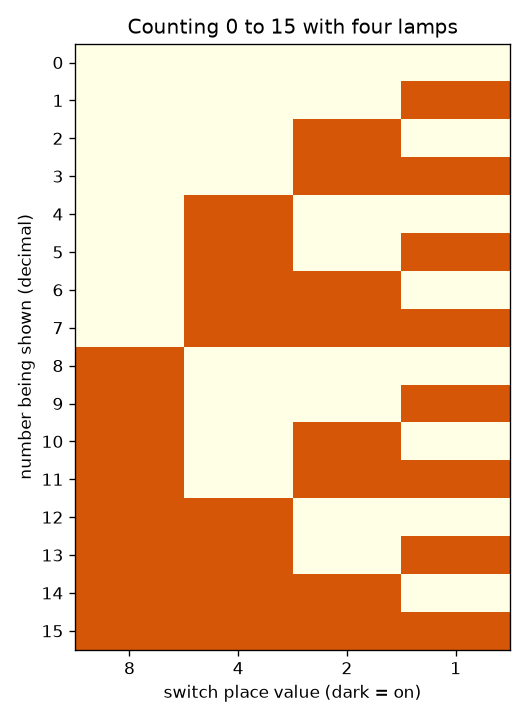
\includegraphics[width=0.85\linewidth]{figures/s01_counting_lamps.png}\\\small Counting 0 to 15: one row per number, dark squares are lamps that are on.\end{center}

\subsection*{E. Worked example}
What number do the switches 1101 show? Then show the number 12 as switches.
\begin{enumerate}[nosep]
\item Write the place values over the switches: 8, 4, 2, 1.
\item Switches on are the first, second and fourth, so add 8 + 4 + 1 and add 0 for the third: 8 + 4 + 0 + 1 = 13.
\item For 12 take the biggest place value that fits: 8 fits (12 - 8 = 4), 4 fits (4 - 4 = 0), 2 and 1 do not.
\item So 12 is 8 + 4 = 1100 (first and second switch on).
\item Check: 8 + 4 + 0 + 0 = 12.
\end{enumerate}
\textbf{Answer.} 1101 shows 13, and 12 is written 1100.

\subsection*{F. Questions}
\begin{enumerate}[nosep]
\item \textbf{Conceptual.} Why does adding one more switch exactly double the number of different patterns?
\item \textbf{Numerical.} Read the switches 1011 as a decimal number, and write 12 as switches. Sanity check each result.
\item \textbf{Graph and simulation interpretation.} In the graph of lamps on against the number, how many numbers between 0 and 15 have exactly two lamps on? What is the highest point of the graph and where does it occur?
\item \textbf{Design and optimisation challenge.} Design: a hall has 100 seats numbered from 0 to 99. A sign should show the seat number on lamps. What is the smallest number of lamps? Name one trade-off of using more lamps than that.
\end{enumerate}

\section{Session 2: Number systems, logic gates and Boolean algebra}

\subsection*{A. Real-world problem}
A stairwell light has a switch at the top and one at the bottom, and either one must toggle the light. A lift must not move unless the door is closed AND the load is within the limit. Rules like these are built from logic gates, tiny circuits whose output is 0 or 1 and depends only on their inputs. To talk about the numbers inside such machines, engineers also write them in hexadecimal, which is binary in a short form. This is a simplified educational model: ideal gates with no electrical detail.

\subsection*{B. Concept and theory}
In base b the digit string d\_k ... d\_1 d\_0 means d\_k b\textasciicircum{}k + ... + d\_1 b + d\_0. To convert a number to base b, divide by b again and again and collect the remainders, last remainder first. Hexadecimal (base 16) uses digits 0 to 9 and A to F (A is 10, F is 15), and each hex digit stands for exactly four bits, so 1011 0111 is B7. A logic gate maps input bits to an output bit. AND gives 1 only if both inputs are 1; OR gives 1 if at least one is 1; NOT flips a bit; XOR gives 1 if the inputs differ; NAND is NOT of AND. A truth table lists the output for every input row, and a claim that is true on every row is proved. De Morgan's laws turn an AND into an OR by flipping inputs and output. Because NAND(a, a) is NOT a, NAND can build NOT, then AND, then OR, then XOR: it is called universal. Any truth table can be turned into a circuit: write one AND term (a minterm) for each row whose output is 1 and OR the terms together (sum of products).

\begin{itemize}[nosep]
\item b: the base of a number system (2, 10 or 16) (no unit)
\item d\_k: digit in place k (no unit)
\item a, b: input bits of a gate (0 or 1)
\item NOT a: the opposite bit of a (written with a bar in equations) (0 or 1)
\item minterm: an AND term that is 1 on exactly one input row (0 or 1)
\end{itemize}

\begin{equation*}
N=\sum_k d_k\,b^{k}
\end{equation*}

\begin{equation*}
\overline{a\cdot b}=\bar a+\bar b,\qquad \overline{a+b}=\bar a\cdot\bar b
\end{equation*}

\begin{equation*}
\bar a=\overline{a\cdot a},\qquad a\cdot b=\overline{\overline{a\cdot b}},\qquad a+b=\overline{\bar a\cdot\bar b}
\end{equation*}

\begin{equation*}
a\oplus b=a\bar b+\bar a b
\end{equation*}

\begin{equation*}
\text{majority}(a,b,c)=\bar a bc+a\bar b c+ab\bar c+abc=ab+ac+bc
\end{equation*}

\begin{center}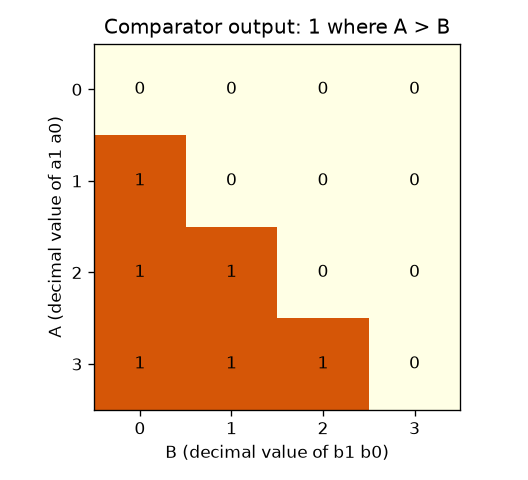
\includegraphics[width=0.85\linewidth]{figures/s02_comparator.png}\\\small The 2-bit comparator: dark where A is greater than B.\end{center}

\subsection*{E. Worked example}
Convert 183 to binary and to hexadecimal, and check by converting back.
\begin{enumerate}[nosep]
\item Divide by 2 repeatedly and collect remainders from last to first. 183 = 128 + 32 + 16 + 4 + 2 + 1, so the bits are 1 0 1 1 0 1 1 1.
\item So 183 is 10110111 in binary.
\item Group in fours from the right: 1011 and 0111. 1011 is 11, which is B, and 0111 is 7.
\item So 183 is B7 in hexadecimal.
\item Check: B7 = 11 x 16 + 7 = 176 + 7 = 183. The same number.
\end{enumerate}
\textbf{Answer.} 183 is 10110111 in binary and B7 in hexadecimal.

\subsection*{F. Questions}
\begin{enumerate}[nosep]
\item \textbf{Conceptual.} Why can NAND build every other gate? Show how to get NOT and OR from NAND.
\item \textbf{Numerical.} Convert the hexadecimal number A5 to decimal and to binary, and convert decimal 100 to binary and hexadecimal. Sanity check.
\item \textbf{Graph and simulation interpretation.} In the comparator figure (A down the side, B along the top, dark where A \textgreater{} B), where are the dark squares and how many are there? Why is the diagonal white?
\item \textbf{Design and optimisation challenge.} Design: a lock opens when the 2-bit number A equals the 2-bit number B. Build the truth table, write the sum-of-products form and give a shorter form with XNOR. How many minterms are there?
\end{enumerate}

\section{Session 3: Build an adder from gates and see how computers count}

\subsection*{A. Real-world problem}
Inside a processor there is no plus button, only gates. Yet it adds very many numbers every second, subtracts, and knows when an answer does not fit. How can a handful of AND, OR and XOR gates add two numbers, and why does it take longer to add 32 bits than 4? We build the arithmetic of a computer from scratch in a tiny simulator and test every circuit against Python's own integers on every possible input. This is a simplified educational model: ideal gates, each with one unit of delay, no clock and no real chip timing.

\subsection*{B. Concept and theory}
A half adder adds two bits: the sum bit is a XOR b (1 when the inputs differ) and the carry bit is a AND b (1 when both are 1). A full adder also takes a carry in: sum = a XOR b XOR c\_in and carry out = ab + (a XOR b) c\_in; it is two half adders and an OR gate, five gates in all. Chain n full adders with the carry out of each feeding the next and you get an n-bit ripple-carry adder. In n-bit two's complement the leftmost bit counts as -2\textasciicircum{}(n-1) instead of +2\textasciicircum{}(n-1), so four bits cover -8 to 7 and 1111 means -1. To negate a number flip every bit and add 1, so a - b = a + (NOT b) + 1: XOR every b bit with a control bit \texttt{sub} and use \texttt{sub} as the carry in, and one adder both adds and subtracts. If the true answer is outside the range, the result wraps round and overflow occurs; it is detected when the carry into the top bit differs from the carry out of it. Each gate takes one unit of delay, and a wire's depth is one more than the depth of its slowest input. The carry out of stage i must wait for the carry out of stage i - 1, so the delay of the last carry grows in a straight line with the width. That is why fast processors use carry-lookahead circuits (a stretch topic) that work out carries in parallel. An ALU (arithmetic logic unit) feeds the same inputs to several operations and a control code selects which result comes out.

\begin{itemize}[nosep]
\item a, b: input bits (or n-bit numbers) (0 or 1)
\item c\_in, c\_out: carry into and out of a stage (0 or 1)
\item n: adder width (bits)
\item sub: control bit: 0 add, 1 subtract (0 or 1)
\item T(n): delay of the last carry out (gate delays)
\item op: ALU control code: 00 add, 01 subtract, 10 AND, 11 OR (2 bits)
\end{itemize}

\begin{equation*}
s=a\oplus b\oplus c_{in},\qquad c_{out}=ab+(a\oplus b)\,c_{in}
\end{equation*}

\begin{equation*}
\text{value}=-b_{n-1}2^{\,n-1}+\sum_{k=0}^{n-2}b_k 2^{k},\qquad -2^{n-1}\le \text{value}\le 2^{n-1}-1
\end{equation*}

\begin{equation*}
a-b=a+\bar b+1\pmod{2^{n}}
\end{equation*}

\begin{equation*}
\text{overflow}=c_{n-1}\oplus c_{n}
\end{equation*}

\begin{equation*}
T(n)=2n+1\ \text{gate delays}
\end{equation*}

\begin{center}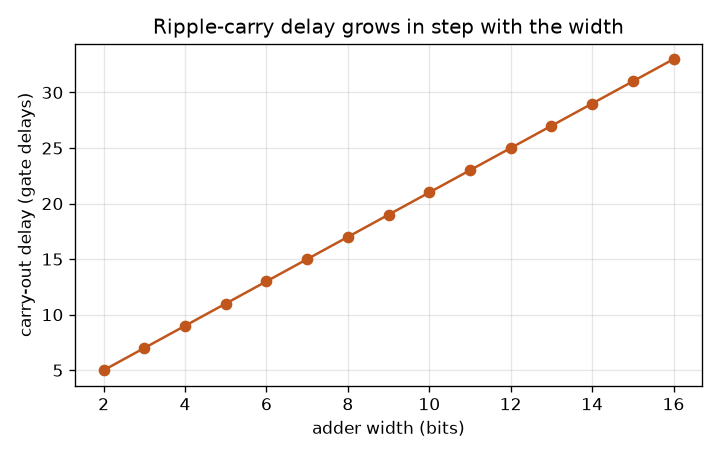
\includegraphics[width=0.85\linewidth]{figures/s03_carry_delay.png}\\\small Carry-out delay of the ripple adder grows in a straight line with its width.\end{center}

\subsection*{E. Worked example}
Compute 6 - 3 on four bits with the adder-subtractor, showing the bits.
\begin{enumerate}[nosep]
\item Subtraction means sub = 1: flip every bit of b and add 1 through the carry in.
\item 6 is 0110 and 3 is 0011; flipping the bits of 3 gives 1100.
\item Add 0110 + 1100 + 1 (the carry in) = 10011.
\item Keep only four bits: 0011, the carry out of the top bit is thrown away.
\item 0011 is 3, and 6 - 3 = 3. The carry into the top bit and the carry out of it are equal, so there is no overflow.
\end{enumerate}
\textbf{Answer.} 6 - 3 = 3, pattern 0011, overflow flag 0.

\subsection*{F. Questions}
\begin{enumerate}[nosep]
\item \textbf{Conceptual.} Why does 7 + 1 give -8 on four bits, and how does the circuit know that the answer is wrong?
\item \textbf{Numerical.} Compute 5 - 7 on four bits: show the three numbers you add, the four-bit result, and whether overflow occurs. Sanity check with ordinary arithmetic.
\item \textbf{Graph and simulation interpretation.} From the delay graph, how many gate delays does the carry take for 8 bits, and for 12 bits? What does the slope of the line tell you?
\item \textbf{Design and optimisation challenge.} Design: each gate takes 0.5 ns and the carry out of a ripple adder must be ready within 20 ns. What is the widest adder allowed? What would you change to go wider?
\end{enumerate}

\section{Session 4: A carry-lookahead adder}

\subsection*{A. Real-world problem}
Session 3 built an adder that is correct for every input, but its carry ripples: the last carry waits for every carry before it, so the delay is 2n + 1 gate delays. A 16-bit ripple adder needs 33 gate delays and a 32-bit one needs 65, far too slow for the adder inside a processor that has to finish in one clock tick. How can an adder get its carries without waiting for them? We work out what each stage will generate and propagate, write every carry in terms of those signals, and build two faster adders in the same simulator. Each is checked against Python's own addition, and we count honestly what the speed costs in gates. This is a simplified educational model: ideal gates with two inputs and one unit of delay each, no wires, no fan-out limit, no clock and no real chip timing.

\subsection*{B. Concept and theory}
Look at one stage with inputs a and b and ask what it does to a carry that arrives. If a = b = 1 it \textbf{generates} a carry whatever arrives: g = a AND b. If a and b differ it \textbf{propagates}: an arriving carry passes straight through, so p = a XOR b. If a = b = 0 it \textbf{kills} an arriving carry, and g = p = 0. The carry out of the stage is c\_next = g OR (p AND c), and the sum bit is p XOR c. The key fact is that g and p use only the stage's own inputs, so they are ready after one gate delay in every stage at once.

Now substitute c\_next = g + p c into itself. For example c4 = g3 + p3 g2 + p3 p2 g1 + p3 p2 p1 g0 + p3 p2 p1 p0 c\_in (+ is OR, writing two symbols together is AND). Every term uses only g, p and the carry in, so all carries can be computed at the same time instead of one after another. At most one term can be 1, because a stage that generates has p = 0 and blocks every term that starts further down. So each carry has exactly one source: a stage that generated it with every stage above it passing it on, or the carry in itself.

With two-input gates an AND of 17 signals still needs 5 levels, and an OR of 17 terms another 5, so lookahead is not instant. The \textbf{flat lookahead adder} builds every term and every OR in full, joining the shallowest wires first; it is the textbook idea with no sharing, fast but expensive in gates. The \textbf{parallel-prefix adder} is smarter. A group of stages has its own generate G and propagate P, and a high group joins the group below it with G = G\_high + P\_high G\_low and P = P\_high P\_low. Joining at distances 1, 2, 4, 8, ... (the Kogge-Stone pattern) makes every stage's group reach back to stage 0 after log2(n) rounds, two gate delays per round, so doubling the width adds exactly 2 gate delays. No circuit of two-input gates can do better than ceil(log2(2n + 1)) levels for the last carry, because that carry depends on all 2n + 1 inputs.

\begin{itemize}[nosep]
\item a, b: input bits of one stage (0 or 1)
\item g, p: generate (a AND b) and propagate (a XOR b) of a stage (0 or 1)
\item c\_in, c\_i: carry in, and carry into stage i (0 or 1)
\item G, P: generate and propagate of a group of stages (0 or 1)
\item n: adder width (bits)
\item T(n): delay of the last carry out (gate delays)
\item gates: number of gates in the circuit (count)
\end{itemize}

\begin{equation*}
g_i=a_ib_i,\qquad p_i=a_i\oplus b_i
\end{equation*}

\begin{equation*}
c_{i+1}=g_i+p_ic_i,\qquad s_i=p_i\oplus c_i
\end{equation*}

\begin{equation*}
c_{i+1}=g_i+p_ig_{i-1}+p_ip_{i-1}g_{i-2}+\dots+p_i\cdots p_0\,c_{in}
\end{equation*}

\begin{equation*}
(G,P)=(G_h+P_hG_l,\;P_hP_l)
\end{equation*}

\begin{equation*}
T_{\text{ripple}}(n)=2n+1,\qquad T_{\text{prefix}}(2^k)=2k+3,\qquad T\ge\lceil\log_2(2n+1)\rceil
\end{equation*}

\begin{center}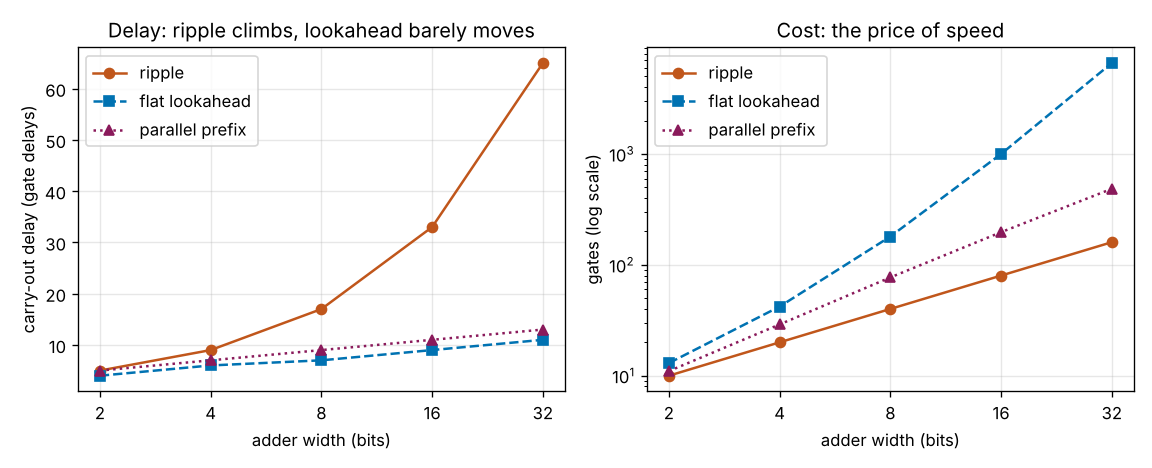
\includegraphics[width=0.95\linewidth]{figures/s04_delay_cost.png}\\\small Carry-out delay and gate count against width: the lookahead adders are much faster and cost more gates.\end{center}

\subsection*{E. Worked example}
Add 11 + 5 on four bits using the lookahead equations, with carry in 0, and say where the last carry comes from.
\begin{enumerate}[nosep]
\item Write the inputs: a = 1011 and b = 0101.
\item Generate g = a AND b = 0001 (only stage 0 has two ones) and propagate p = a XOR b = 1110 (stages 1, 2 and 3 have one 1 each).
\item All the carries from the equations: c1 = g0 + p0 c\_in = 1 + 0 = 1; c2 = g1 + p1 g0 + p1 p0 c\_in = 0 + 1 + 0 = 1; c3 = g2 + p2 g1 + p2 p1 g0 + ... = 0 + 0 + 1 = 1; c4 = g3 + p3 g2 + p3 p2 g1 + p3 p2 p1 g0 + ... = 0 + 0 + 0 + 1 = 1.
\item The sum bits are s\_i = p\_i XOR c\_i, with c\_0 = c\_in = 0: s0 = 0 XOR 0 = 0, s1 = 1 XOR 1 = 0, s2 = 1 XOR 1 = 0, s3 = 1 XOR 1 = 0.
\item The result is 0000 with carry out 1, which is 16, and 11 + 5 = 16. The only term of c4 that is 1 is p3 p2 p1 g0: stage 0 generated the carry and stages 1, 2 and 3 passed it on.
\end{enumerate}
\textbf{Answer.} 11 + 5 = 16: sum bits 0000, carry out 1, and the last carry comes from stage 0.

\subsection*{F. Questions}
\begin{enumerate}[nosep]
\item \textbf{Conceptual.} Why can a lookahead adder find the carry out of stage 3 without waiting for the carries out of stages 0, 1 and 2? What do generate and propagate mean?
\item \textbf{Numerical.} Use the equations to find the carry out of stage 3 (c4) for a = 1101 (13) and b = 0111 (7) with carry in 0. Which stage did it come from? Sanity check with ordinary addition.
\item \textbf{Graph and simulation interpretation.} From the delay graph, how many gate delays does the carry out take at 16 bits and at 32 bits for the ripple, flat and prefix adders? What happens to each when the width doubles?
\item \textbf{Design and optimisation challenge.} Design: a 32-bit adder must have its carry out ready within 7.5 ns at 0.5 ns per gate delay, using at most 1000 gates. Which of the ripple, flat and prefix designs would you choose? What would change if the budget were 10 gate delays?
\end{enumerate}

\section{Session 5: A multiplier from gates}

\subsection*{A. Real-world problem}
The adder of Session 3 can add and subtract, but a processor also has to multiply: to scale a sound, to mix colours, to work out an address. There is no multiply gate. Yet two 4-bit numbers can be multiplied with nothing more than AND gates and the half and full adders we already have. How, and what does it cost? We build the multiplier in the gate simulator, test it on all 256 input pairs against Python's own multiplication, and then ask how many gates it needs, how long its slowest product bit takes, and why the answer needs twice as many bits as the inputs. This is a simplified educational model for unsigned numbers: ideal gates with one unit of delay each, no wires, no clock and no real chip timing.

\subsection*{B. Concept and theory}
Multiplying on paper, you multiply the top number by each digit of the bottom number and add the rows, each shifted one place further left. In binary every digit is 0 or 1, so each row is either 0 or a copy of a, shifted: row j is a x b\_j shifted j places. These rows are the partial products. Bit i of row j is a\_i AND b\_j, so a 4 x 4 multiplier makes its 16 partial-product bits with 16 AND gates, all at once. The rows are then added column by column: in each column add the ones that fall in it and the carry from the column before, write the last bit of the total and carry the rest. On paper a carry can be as big as 3 for 4 bits; in the circuit each half adder (two bits) or full adder (two bits and a carry) passes on a single carry bit, and a bit alone in its column passes straight through.

Adding the rows one after another with a regular grid of adder cells gives the \textbf{array multiplier}. Each row after the first needs n cells: n half adders and n(n - 2) full adders in all for an n x n multiplier, plus the n\textasciicircum{}2 AND gates, so the gate count is 6n\textasciicircum{}2 - 8n. It grows with the square of the width: doubling n multiplies the gates by more than 4 (5 from 4 to 8 bits), tending to 4 for wide multipliers. The slowest path runs down through the rows and across, and in the simulator it takes 6n - 8 gate delays for n \textgreater{}= 3, growing in step with n. Because a and b are each at most 2\textasciicircum{}n - 1, the product is at most (2\textasciicircum{}n - 1)\textasciicircum{}2 which is below 2\textasciicircum{}(2n): it needs 2n bits and cannot overflow if you keep them all. A narrow chip that keeps only the low n bits gets most answers wrong: 15 x 15 = 225 becomes 1 on four bits.

\begin{itemize}[nosep]
\item a, b: the two unsigned inputs (n-bit numbers)
\item a\_i, b\_j: bit i of a and bit j of b (0 or 1)
\item n: width of each input (bits)
\item pp\_j: partial product j: a shifted left j places if b\_j is 1, else 0 (number)
\item p: the product a x b, 2n bits wide (2n-bit number)
\item T(n): delay of the slowest product bit (gate delays)
\end{itemize}

\begin{equation*}
a\times b=\sum_{j=0}^{n-1} b_j\,(a\ll j),\qquad \text{bit } i \text{ of row } j = a_i\wedge b_j
\end{equation*}

\begin{equation*}
0\le a\times b\le (2^n-1)^2<2^{2n}
\end{equation*}

\begin{equation*}
\text{gates}(n)=n^2+2n+5\,n(n-2)=6n^2-8n
\end{equation*}

\begin{equation*}
T(n)=6n-8\ \text{gate delays}\quad(n\ge 3)
\end{equation*}

\begin{center}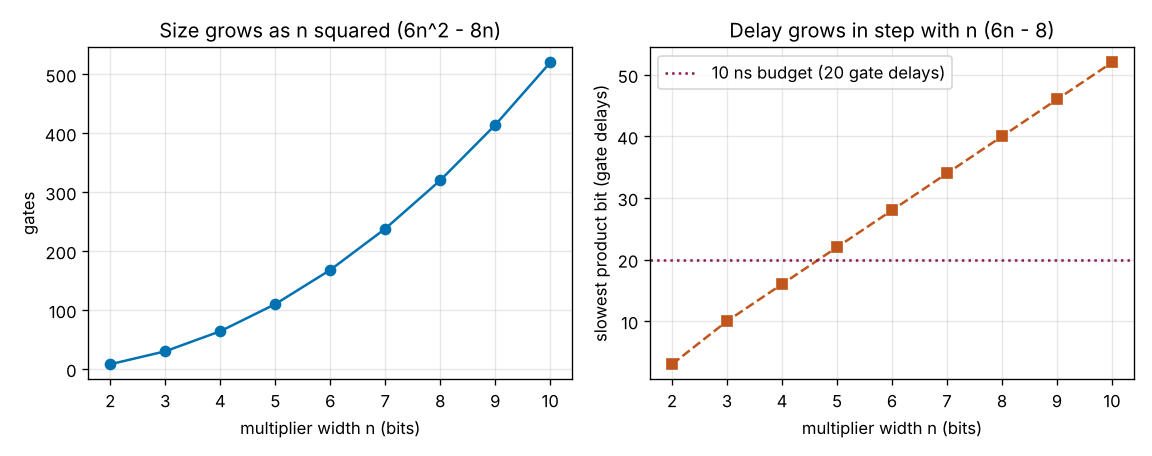
\includegraphics[width=0.95\linewidth]{figures/s05_size_delay.png}\\\small Gates grow with n squared and delay grows in step with n.\end{center}

\subsection*{E. Worked example}
Multiply 7 x 3 with the AND-gate partial products and the column method, and check the answer.
\begin{enumerate}[nosep]
\item Write the inputs: a = 0111 and b = 0011, so b0 = 1 and b1 = 1 and the other bits of b are 0.
\item The partial products are row 0 = a = 0111 and row 1 = a shifted one place = 01110; rows 2 and 3 are all zeros.
\item Column 0: only a0 AND b0 = 1, so the product bit is 1. Column 1: a1b0 = 1 and a0b1 = 1, two ones, total 2, so bit 0 and carry 1.
\item Column 2: a2b0 = 1 and a1b1 = 1 plus the carry 1, total 3, so bit 1 and carry 1. Column 3: a2b1 = 1 plus the carry 1, total 2, so bit 0 and carry 1.
\item Column 4: no ones plus the carry 1, total 1, so bit 1; the higher columns are 0. Reading the bits from column 7 down gives 00010101.
\end{enumerate}
\textbf{Answer.} 7 x 3 = 00010101 = 21, and 7 x 3 = 21 in ordinary arithmetic.

\subsection*{F. Questions}
\begin{enumerate}[nosep]
\item \textbf{Conceptual.} Why does the product of two 4-bit numbers need 8 bits, and why does multiplying by 8 need no adder at all?
\item \textbf{Numerical.} Multiply 13 x 11 by partial products: write each row, add them, and give the product in binary. Sanity check with decimal arithmetic.
\item \textbf{Graph and simulation interpretation.} From the size and delay graph, how many gates and how many gate delays does the multiplier have at n = 4 and at n = 8? What happens to each when the width doubles?
\item \textbf{Design and optimisation challenge.} Design: each gate takes 0.5 ns and the product of an array multiplier must be ready within 10 ns. What is the widest multiplier allowed? What would you change to go wider?
\end{enumerate}

\section{Real-world mini-project}
\textbf{Build and test an 8-bit adder-subtractor.} A small calculator chip needs to add and subtract 8-bit numbers (-128 to 127) and to warn when the answer does not fit. Use \texttt{build\_add\_sub(8)} and \texttt{add\_sub} from Session 3. Test it on every pair of inputs for both operations against Python integers, count the pairs that overflow, count its gates, read the delay of its overflow flag, and then decide the widest adder-subtractor whose overflow flag is ready within a 10 ns budget if one gate takes 0.5 ns.

\textbf{Choose the adder for a 32-bit processor.} A small processor needs a 32-bit adder whose carry out must be ready within 7.5 ns, at 0.5 ns per gate delay (15 gate delays), and the chip area allows at most 1000 gates for the adder. Use \texttt{build\_ripple}, \texttt{build\_flat} and \texttt{build\_prefix} from Session 4 at 32 bits. Check each design against Python, read its gates and carry-out delay, convert the delay to nanoseconds, and decide which design meets both budgets. \textbf{Deliverable:} A script that builds the three 32-bit adders, checks each against Python on 20000 random pairs plus corner cases and the prefix adder on 200000, prints a table of gates, carry-out delay and time in nanoseconds, prints which designs meet 15 gate delays and 1000 gates, finds the widest ripple adder within 15 gate delays, and saves a picture of the delay and gate curves. \textbf{Success looks like:} No mismatches in any check. The table shows ripple 160 gates, 65 gate delays, 32.5 ns; flat 6608 gates, 11 gate delays, 5.5 ns; prefix 485 gates, 13 gate delays, 6.5 ns. Only the prefix adder meets both budgets (ripple is too slow, flat uses too many gates), the widest ripple adder within 15 gate delays is 7 bits, and the prefix adder is 5 times faster than ripple (65 / 13) for about 3 times the gates (485 / 160).

\textbf{Build and test an 8 x 8 multiplier.} A small calculator chip must multiply two 8-bit unsigned numbers (0 to 255) and show the result. Use \texttt{build\_multiplier(8)}, \texttt{multiply} and \texttt{mismatches} from Session 5. Test it on every pair of inputs against Python's \texttt{*}, count its gates, read the delay of its slowest product bit, count how many of the 65536 products do not fit in 8 bits, and decide the widest array multiplier whose slowest product bit is ready within 20 ns if one gate takes 0.5 ns. \textbf{Deliverable:} A script that checks all 65536 input pairs against Python, prints the number of gates, the number of product bits, the delay of the slowest product bit in gate delays and in ns, the number of products above 255, and the widest width that meets the 20 ns budget, and saves a picture of the gates and delay against n. \textbf{Success looks like:} Every one of the 65536 pairs matches Python, the multiplier has 320 gates and 16 product bits, the slowest product bit is ready after 40 gate delays (20 ns), 63568 of the 65536 products (97.0 \%) are above 255 and so need more than 8 bits, and the widest width within 20 ns is 8 bits (a 9-bit multiplier needs 46 gate delays, 23 ns).

\section{The path ahead}
\begin{enumerate}[nosep]
\item \textbf{Session 6: A saturating adder.} An 8-bit adder-subtractor that returns the nearest extreme on overflow.
\item \textbf{Session 7: A counter that remembers.} A 4-bit counter driven by clock ticks.
\item \textbf{Session 8: An ALU with flags and a decoder.} An 8-bit ALU with four operations and flags, and a decoder lighting the right segments for each digit.
\end{enumerate}

\section{Answers and hints}

\subsection*{Session 1}
\begin{enumerate}[nosep]
\item \textbf{Conceptual.} Hint: Take every pattern you already had and ask how many ways the new switch can be set. Solution: Each old pattern can be combined with the new switch off or on, which gives two new patterns for every old one. Four switches make 16 patterns, five make 32. So n switches make 2\textasciicircum{}n patterns, and the largest number is 2\textasciicircum{}n - 1 because the counting starts at 0.
\item \textbf{Numerical.} Hint: Use the place values 8, 4, 2, 1. Solution: 1011 = 8 + 0 + 2 + 1 = 11. For 12: 8 + 4 = 12, so the pattern is 1100. Sanity check: 11 is below 15 (the largest on 4 switches) and 1100 sums back to 12.
\item \textbf{Graph and simulation interpretation.} Hint: Count the dots at height 2, and look for the number with every switch on. Solution: Six numbers have exactly two lamps on: 3, 5, 6, 9, 10 and 12. The graph is highest (4 lamps) at 15, where every switch is on, and lowest (0 lamps) at 0. The counts at heights 0 to 4 are 1, 4, 6, 4, 1.
\item \textbf{Design and optimisation challenge.} Hint: Find the smallest n with 2\textasciicircum{}n at least 100. Solution: 6 lamps give only 64 patterns, which is not enough. 7 lamps give 128 patterns, which covers 0 to 99, so 7 lamps are enough and 7 is the smallest number. Using 8 or more lamps would cost more parts and more wiring while only wasting patterns; using fewer is impossible. Assumption: one lamp per bit and a fixed, known maximum seat number.
\end{enumerate}

\subsection*{Session 2}
\begin{enumerate}[nosep]
\item \textbf{Conceptual.} Hint: What does NAND do when both inputs are the same wire? Then use De Morgan. Solution: NAND(a, a) is NOT(a AND a) = NOT a, so NAND gives NOT. AND is NOT of NAND, so AND takes two NAND gates. OR(a, b) = NOT(NOT a AND NOT b) = NAND(NOT a, NOT b), which takes three NAND gates. XOR takes four. With NOT and AND you can build any truth table, so NAND alone is enough.
\item \textbf{Numerical.} Hint: A is 10. Each hex digit is four bits. Solution: A5 = 10 x 16 + 5 = 165, and A = 1010, 5 = 0101, so A5 is 10100101. For 100: 64 + 32 + 4 = 100, so it is 1100100 in binary; grouping 0110 0100 gives 64 in hexadecimal (6 x 16 + 4 = 100). Check: 10100101 = 128 + 32 + 4 + 1 = 165.
\item \textbf{Graph and simulation interpretation.} Hint: On the diagonal A and B are equal. Solution: There are six dark squares, all below the diagonal (the row number A is larger than the column number B): 3 + 2 + 1 = 6. The diagonal is white because there A = B, so A \textgreater{} B is false. The squares above the diagonal are white because there B is larger.
\item \textbf{Design and optimisation challenge.} Hint: List the 16 rows (a1 a0 b1 b0) and mark those with A = B. XNOR is 1 when its inputs are the same. Solution: A = B on four rows: 0000, 0101, 1010, 1111, so there are 4 minterms out of 16. Sum of products: the OR of those four 4-input AND terms. Shorter: (a1 XNOR b1) AND (a0 XNOR b0), because A = B exactly when each bit pair matches. Trade-off: the sum of products is mechanical and always works, the short form uses fewer gates but needs insight. We checked both on all 16 rows.
\end{enumerate}

\subsection*{Session 3}
\begin{enumerate}[nosep]
\item \textbf{Conceptual.} Hint: Write 0111 + 0001, and compare the carry into the top bit with the carry out of it. Solution: 0111 + 0001 = 1000. Read as two's complement, 1000 is -8, because the top bit has the weight -8. The true answer 8 does not fit in -8 to 7, so the result wrapped round. The carry into the top bit is 1 but the carry out of it is 0; they differ, so the overflow flag is 1.
\item \textbf{Numerical.} Hint: Flip the bits of 7 (0111), add 0101 and add the carry in 1. Solution: NOT 0111 = 1000. Add 0101 + 1000 + 1 = 1110 (14). Read as two's complement, 1110 is 14 - 16 = -2. Check: 5 - 7 = -2, and -2 is inside -8 to 7, so overflow is 0.
\item \textbf{Graph and simulation interpretation.} Hint: The line is T(n) = 2n + 1. Solution: For 8 bits T = 17 gate delays; for 12 bits T = 2 x 12 + 1 = 25. The slope is 2 gate delays per extra bit, the two gates (AND then OR) that the carry passes through in every stage. Doubling the width roughly doubles the delay, which is the reason for carry-lookahead.
\item \textbf{Design and optimisation challenge.} Hint: Solve (2n + 1) x 0.5 \textless{}= 20. Solution: (2n + 1) x 0.5 \textless{}= 20 gives 2n + 1 \textless{}= 40, so n \textless{}= 19.5 and the widest is 19 bits (39 gate delays = 19.5 ns; 20 bits would need 41 gate delays = 20.5 ns). To go wider, use a carry-lookahead adder, or split the work over two clock cycles. Trade-off: lookahead needs more gates for less delay.
\end{enumerate}

\subsection*{Session 4}
\begin{enumerate}[nosep]
\item \textbf{Conceptual.} Hint: Write c4 with the substitution c\_next = g + p c, and see which signals it uses. Solution: A stage generates a carry when a = b = 1 (g = a AND b) and propagates one when a and b differ (p = a XOR b); both depend only on that stage's own inputs, so every stage has them after one gate delay. Substituting c\_next = g + p c again and again gives c4 = g3 + p3 g2 + p3 p2 g1 + p3 p2 p1 g0 + p3 p2 p1 p0 c\_in. This uses only g, p and the carry in, never c1, c2 or c3, so it can be built next to them instead of after them. The price is more gates.
\item \textbf{Numerical.} Hint: First find g = a AND b and p = a XOR b, bit by bit. Solution: a = 1101 and b = 0111, so g = 0101 (stages 0 and 2 have two ones) and p = 1010 (stages 1 and 3 have one 1). Then c4 = g3 + p3 g2 + p3 p2 g1 + p3 p2 p1 g0 + p3 p2 p1 p0 c\_in = 0 + 1 + 0 + 0 + 0 = 1, and the term that is 1 is p3 g2: stage 2 generated a carry and stage 3 passed it on. Check: 13 + 7 = 20 = 16 + 4, so there is a carry out of the top stage and the four sum bits are 0100.
\item \textbf{Graph and simulation interpretation.} Hint: Read the three lines at 16 and at 32 and subtract. Solution: At 16 bits: ripple 33, flat 9, prefix 11. At 32 bits: ripple 65, flat 11, prefix 13. Doubling the width from 16 to 32 adds 32 gate delays to the ripple adder (it nearly doubles, since T = 2n + 1) but only 2 to each lookahead adder, because one more round of combining is enough. So the gap between ripple and lookahead keeps widening with the width.
\item \textbf{Design and optimisation challenge.} Hint: Convert the time to gate delays first: 7.5 / 0.5. Solution: 7.5 / 0.5 = 15 gate delays. Ripple takes 65 (160 gates), so it is too slow. Flat takes 11 gate delays but 6608 gates, so it is too big. Prefix takes 13 gate delays with 485 gates, so only the prefix adder meets both limits. With a budget of 10 gate delays none of the three designs works at 32 bits (the fastest, flat, needs 11), so you would have to narrow the adder (flat at 16 bits needs 9) or find a different design; even then no circuit of two-input gates can beat ceil(log2 65) = 7 levels for a 32-bit carry out.
\end{enumerate}

\subsection*{Session 5}
\begin{enumerate}[nosep]
\item \textbf{Conceptual.} Hint: Find the largest product, and write 8 in binary. Solution: The largest 4-bit number is 15, and 15 x 15 = 225, which is above 15 and needs 8 bits (225 = 11100001). In general (2\textasciicircum{}n - 1)\textasciicircum{}2 is below 2\textasciicircum{}(2n), so 2n bits are always enough and never overflow. Eight is 1000 in binary, so only b3 is 1 and only one partial product is not zero: it is a shifted left three places. There is nothing to add, so multiplying by a power of two is just a shift, which needs wires and no adder.
\item \textbf{Numerical.} Hint: 13 is 1101 and 11 is 1011; the rows come from the 1 bits of 11 (b0, b1 and b3). Solution: b = 1011 has b0 = 1, b1 = 1, b2 = 0 and b3 = 1. The rows are 1101 (13), 11010 (26), 0 and 1101000 (104). Adding: 13 + 26 = 39 and 39 + 104 = 143, which is 10001111 in binary (128 + 8 + 4 + 2 + 1). Check: 13 x 11 = 143.
\item \textbf{Graph and simulation interpretation.} Hint: Read both curves at n = 4 and n = 8 and divide. Solution: At n = 4 there are 64 gates and the slowest bit takes 16 gate delays; at n = 8 there are 320 gates and 40 gate delays. Doubling the width multiplies the gates by 5 (more than 4, tending to 4, because the gates grow with n squared: 6n\textasciicircum{}2 - 8n) and the delay by 2.5 (more than 2, tending to 2, because the delay grows in step with n: 6n - 8). So width is expensive in size and fairly gentle in delay.
\item \textbf{Design and optimisation challenge.} Hint: Solve (6n - 8) x 0.5 \textless{}= 10, using T(n) = 6n - 8. Solution: 10 / 0.5 = 20 gate delays, and 6n - 8 \textless{}= 20 gives n \textless{}= 4.67, so the widest is 4 bits (16 gate delays = 8 ns; 5 bits needs 22 gate delays = 11 ns). To go wider, use faster adders in the rows (the carry-lookahead adders of Session 4 shorten the carry chain), add the partial products in a tree of adders instead of one row after another, or give the multiplier two clock cycles. The trade-off is more gates and a more complicated layout for less delay.
\end{enumerate}

\section{How to join}
Read \texttt{CONTRIBUTING.md} in the repository, then pick an issue labelled \texttt{good first issue}. Repository: \url{https://github.com/KrunalPanchal1995/pan-iit-oss/tree/main/openbinary}

\end{document}
